\documentclass{article}
\usepackage{fontspec}
\usepackage{polyglossia}
\setdefaultlanguage{french}
\usepackage[a4paper,margin=3cm]{geometry}

\usepackage{amsmath}
\usepackage{amssymb}
\usepackage{array}
\usepackage{auto-pst-pdf}
\usepackage{booktabs}
\usepackage{cite}
\usepackage{graphicx}
\usepackage{lmodern}
\usepackage{marvosym}
\usepackage{mathrsfs}
\usepackage{minted}
\usepackage{multicol}
\usepackage{multirow}
\usepackage{paralist}
\usepackage{schemabloc}
\usepackage{siunitx}
\usepackage{soul}
\usepackage{tikz}
\usepackage[european,cuteinductors,siunitx]{circuitikz}
\usepackage{url,hyperref}
\usepackage{verbatim}
\usepackage{xunicode,xltxtra}

\title{
\includegraphics{../../../images/inp-enseeiht.png} \\ ~  \\ ~ \\ ~ \\ ~ \\ Conception of Analog Circuits}
\author{François Pierron \& Guilhem Saurel}
\date{\oldstylenums{\today}}

\begin{document}

\begin{titlepage}
    \setcounter{page}{0}
    \maketitle
    \vfill
    \tableofcontents
    \thispagestyle{empty}
\end{titlepage}

\section*{Introduction}

The goal of this exercise is to design an frequency multiplier, which will have to transform a 50Hz square input into a 400Hz square output.

~

As this is the only thing our client asked for now, we will probably have to define with him a few more things, like the tolerances on these values.

~

The general architecture of our Phase Locked Loop will be this one:

\begin{center}\begin{circuitikz} \draw
    (0,0) node[mixer] (mix) {}
    (2,0) node[draw, minimum size=2em] (lpf) {Low Pass Filter}
    (6,0) node[draw, minimum size=2em] (vco) {Voltage Controlled Oscillator}
    (3,-1) node[draw, minimum size=2em] (fd) {Frequency Divider}
    (-1,0) node[anchor=east] {$f_{in} = 50Hz$} -- (mix.in 1)
    (mix.out) -- (lpf.west)
    (fd.west) -- (0,-1) -- (mix.in 2)
    (lpf.east) -- (vco.west)
    (vco.east) -- (9,0) node[anchor=west] {$f_{out} = 400Hz$}
    (vco.south) -- (6,-1) -- (fd.east)
; \end{circuitikz}\end{center}

\section{Voltage Controlled Oscillator}

As we work at low frequencies (less than 500 Hz), our VCO will be built with two operationnal amplifiers

\subsection{Operationnal Amplifier}

We choose to use a current source of 20 mA. The bias voltage will came from the outside of this hierarchical block because it will
be shared between all the operationnal amplifiers of the PLL.

~

In order to improve the current copy, we need transistors with big lengths, as L drives the slope of the characteristic.

~

We need an output range  greater than 2.5V, in order to crop it later, so we add another transistor in parallel to improve the current of the output level.

~

Next, we tune the Widths and the Lengths of the transistors in order to try to have a mean at about 2.5V, so that when we will
close the loop, the voltages in the drain and the load will be close.

~

The first cutoff frequency is linked to the capacitor, so it must be small enough to have a cutoff frequency higher than 500Hz.

But we may come back on this later, because all that we need is a band-gain product, and we may work with a gain which is not the maximum one.

~

Eventually, we must have a phase margin greater than 60°.

~

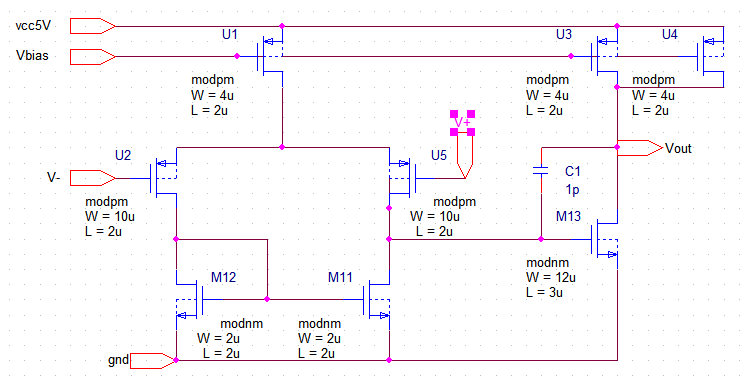
\includegraphics[width=15cm]{AOP.png}

~

With that block, we need a testbench:

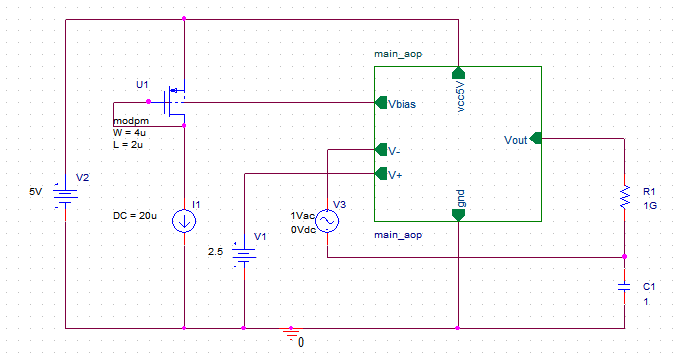
\includegraphics[width=15cm]{test_AOP.png}

~

We can now check our bias voltages and currents:

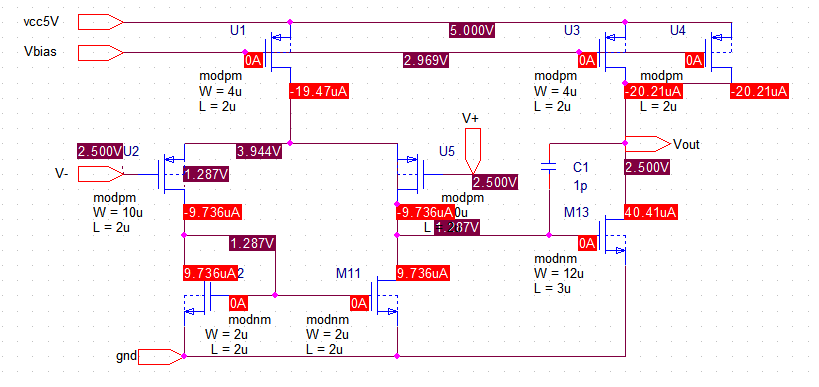
\includegraphics[width=15cm]{bias_AOP.png}

~

With this operationnal amplifier, we achieve those performances :

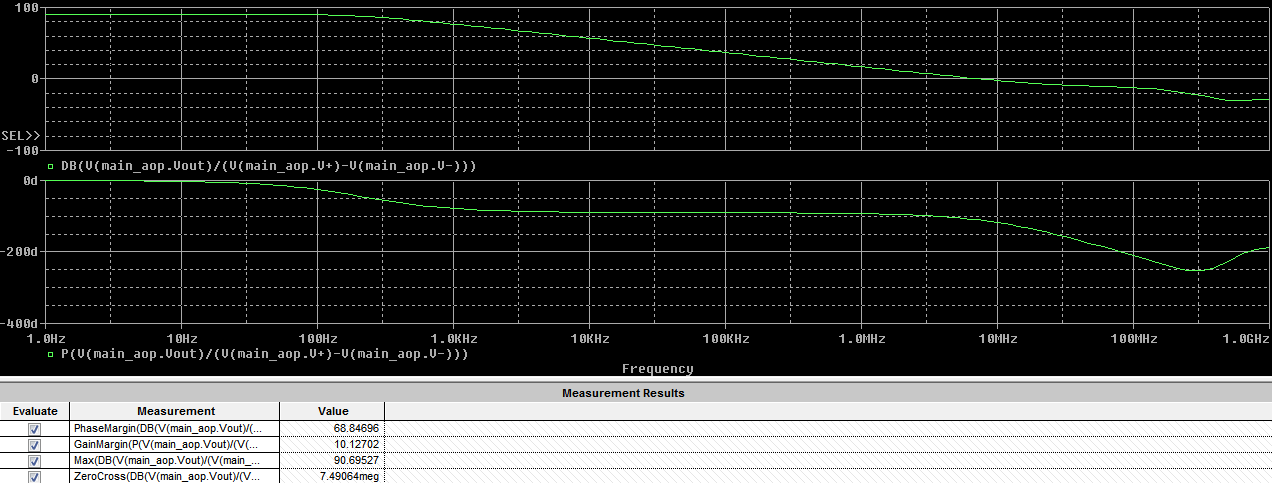
\includegraphics[width=15cm]{bode_aop.png}

\subsection{Voltage controlled oscillator with those operationnal amplifiers}

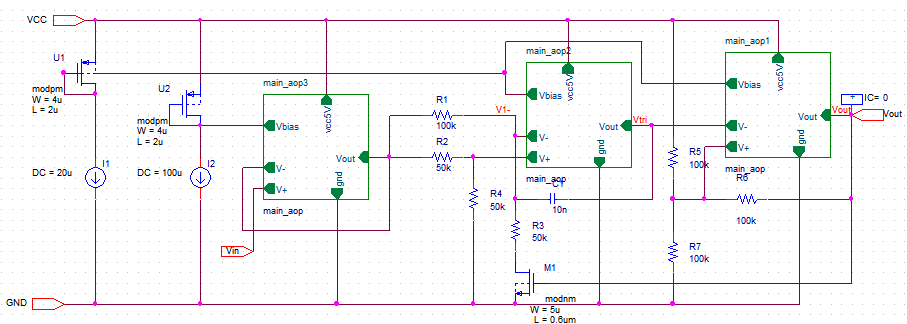
\includegraphics[width=15cm]{VCO_schema.png}

Here, the main problem is about ploting the simulation. We fixed that problem with a simulation of a parametric input voltage, then we can calculate 1 over the Period to get the frequency as a function of the input voltage.

~

We see that we have an output frequency of 400Hz at 1.6V, so we just have to adjust the capacitor to get this frequency at 2.5V.

~

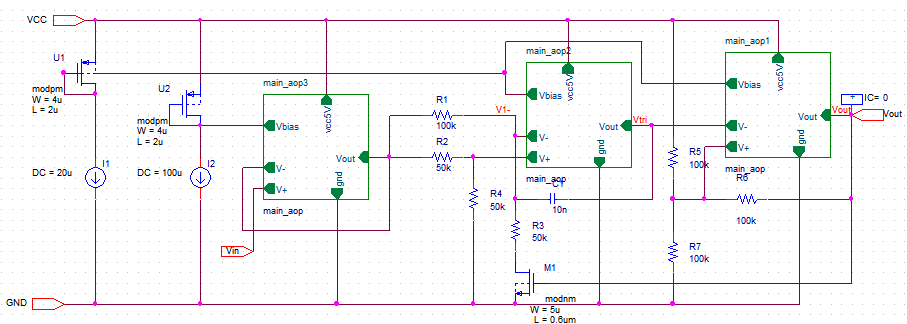
\includegraphics[width=15cm]{VCO_schema.png}

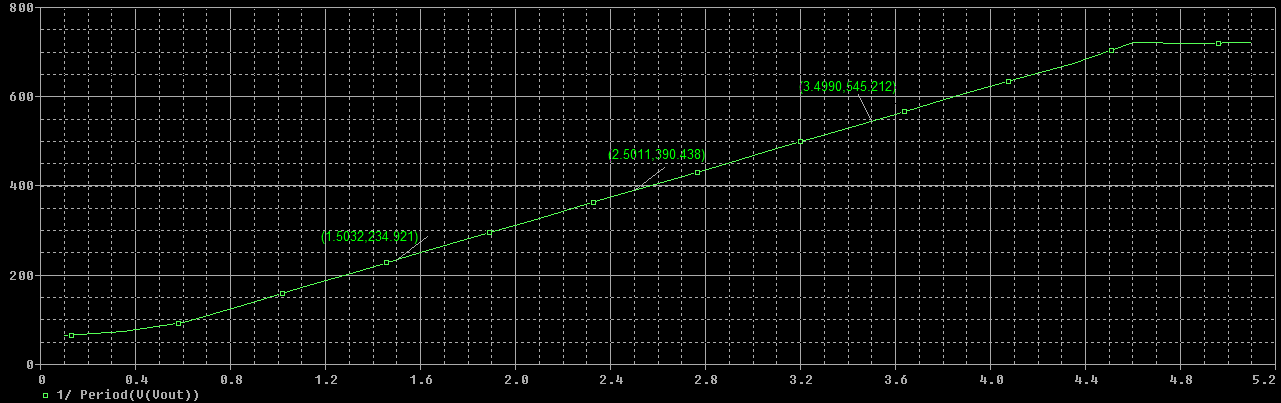
\includegraphics[width=15cm]{VCO_reponse.png}

\section{Divider}

Once the VCO works, we need a frequency divider in the loopback. The easiest way to get a square signal at 50Hz from a square signal at 400Hz is to use three D flip flop.

We could use one of the flip-flop in the librairies, but it would not be fun enough, so we implemented our one, with a few transistors gathered in gates.

\subsection{Inverting Gate}

In this gate, we need a PMOS with a W/L three times bigger than the NMOS.

\subsection{NAND}

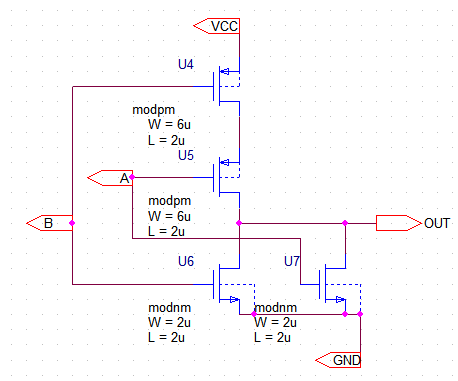
\includegraphics[width=5cm]{nor.png}

\subsection{NOR}

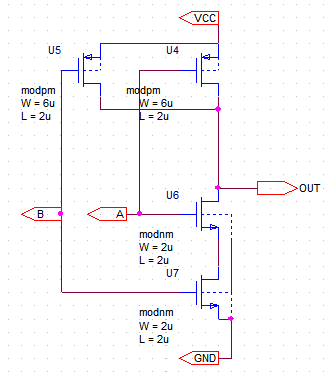
\includegraphics[width=5cm]{nand.png}

\subsection{RS flip-flop}

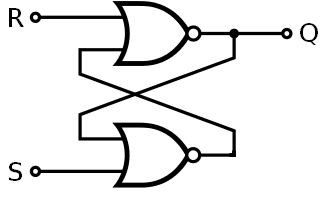
\includegraphics[width=5cm]{bascule_RS.png}

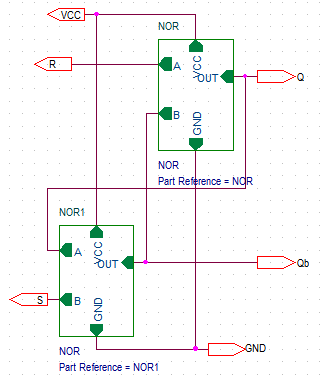
\includegraphics[width=5cm]{RS.png}

Now, we can check that all those logic gates work as expected:

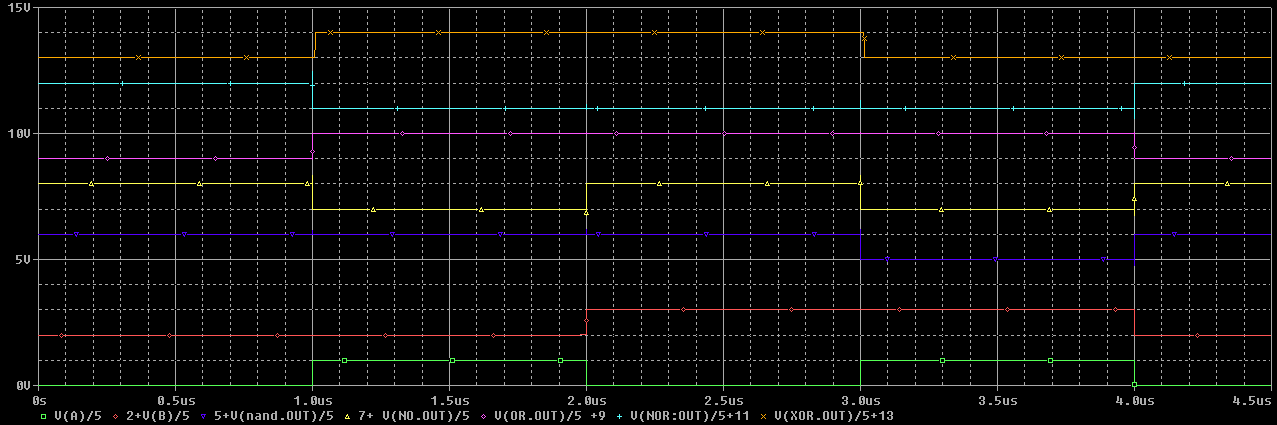
\includegraphics[width=15cm]{test_logic.png}

\subsection{D flip-flop}

With all those logic gates, we can build a D flip-flop:

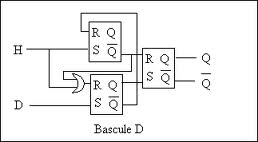
\includegraphics[width=5cm]{basculeD.png}

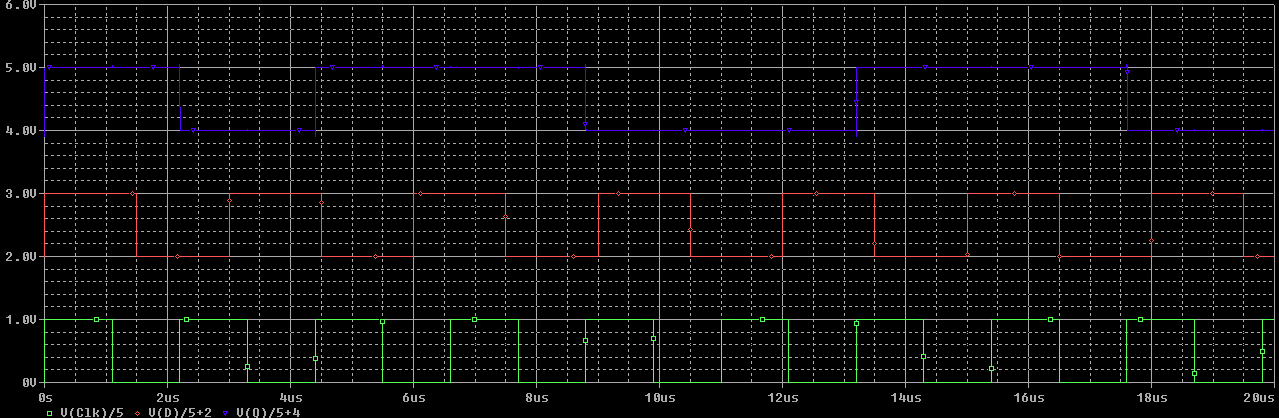
\includegraphics[width=15cm]{test_bascule_D.png}

\section{Comparator}

Here, we need to compare the phase from the input signal with the one coming from the output of D flip flops. Both signals have a 50\% duty cycle and a 5V amplitude, so we can use a simple XOR gate designed earlier.

\section{Low Pass Filter}

Here, we need a really simple Low Pass filter, so we just use a RC filter.

\section{Results}

Here is the first results we got before the changes made by the client:

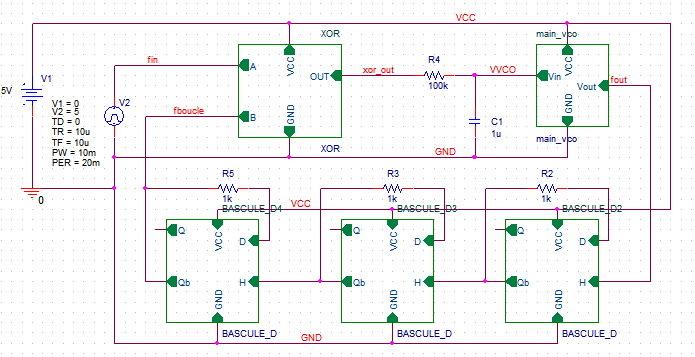
\includegraphics[width=15cm]{pll_first_schematic.png}

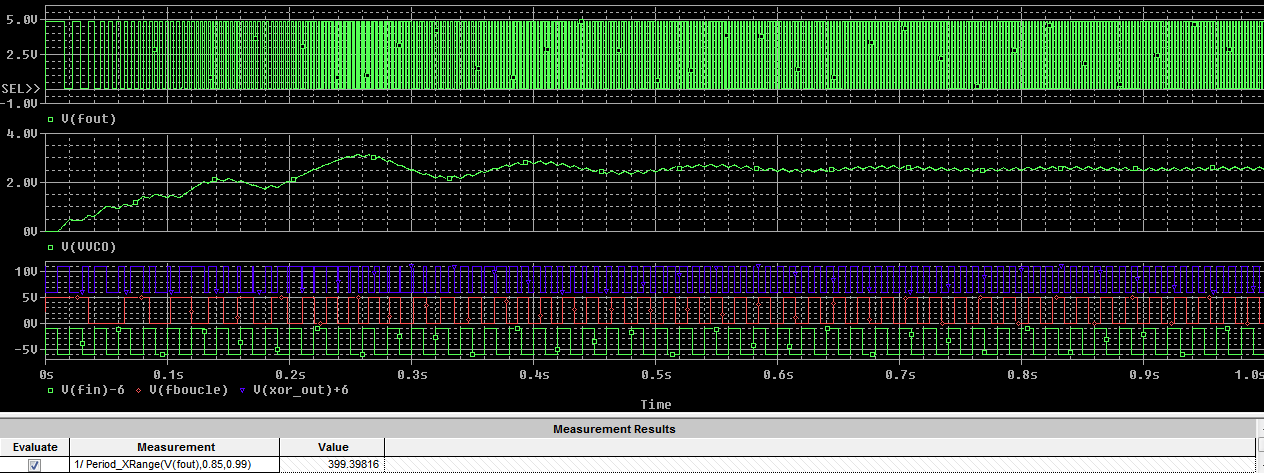
\includegraphics[width=15cm]{pll_first.png}

We can see the PLL catches the input signal, and that the output frequency is quite good.

This output frequency reminds us that we have to define the tolerances, so we proposed 1 \% to our client.


\section{Changes in the needs of the client}

\subsection{Pulse width of the input signal}

The input signal was a square of 50\% pulse width, but now the client needs another pulse width.

~

It does not changes anything for us if we add a D flip-flop before the mixer, because the rising edges of the input will stay at 50Hz.

And as we now have an input of the mixer at 25Hz, we need to add another D flip-flop in the loopback, and we are done.

We also could use an other phase comparator, based on D flip flop, which do not care of the input pulse-with.

\subsection{Sinus Output}

Now, the client needs a sinusoidal output. The solution is once again quite strait-forward, as we just need a big low-pass filter to reject the harmonics.

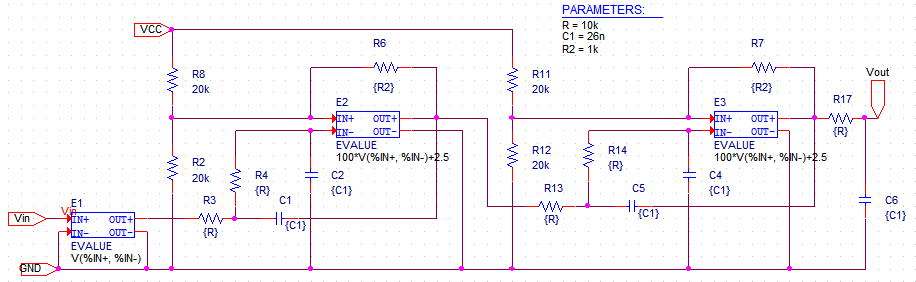
\includegraphics[width=15cm]{filtre_sortie.png}

This is a fifth order low pass filter, where AOP are modelised with "EVALUE" components.

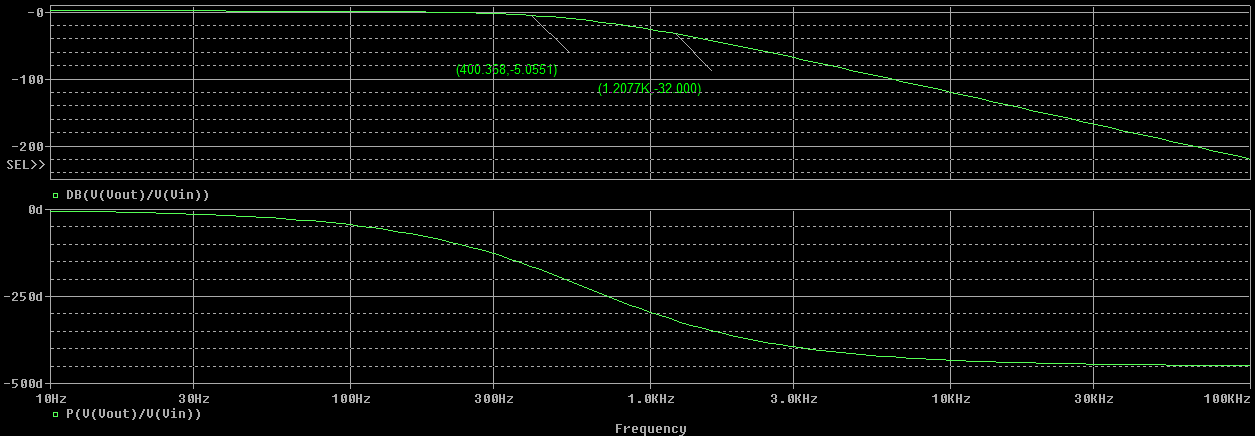
\includegraphics[width=15cm]{bode_filtre_sortie.png}

We can now check that the output is a sinus by checkint its Fast Fourrier Transform:

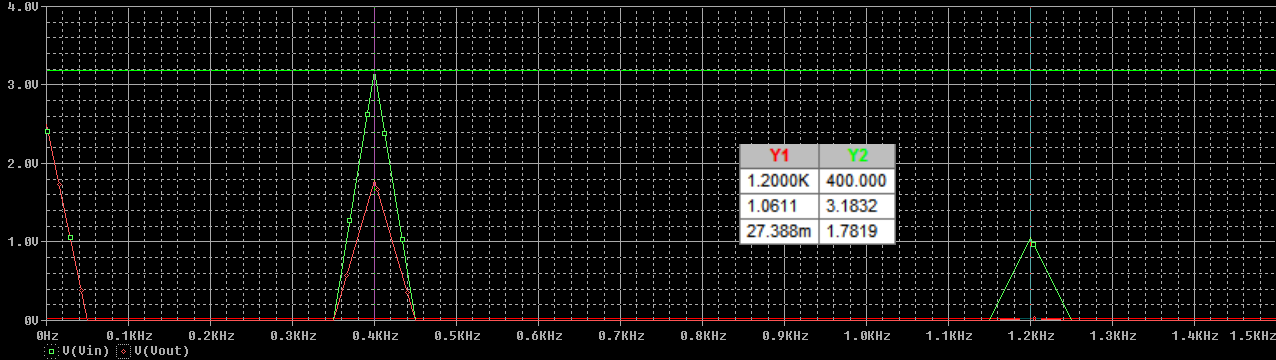
\includegraphics[width=15cm]{fft_filtre_sortie.png}


Then, with the new needs of the client:

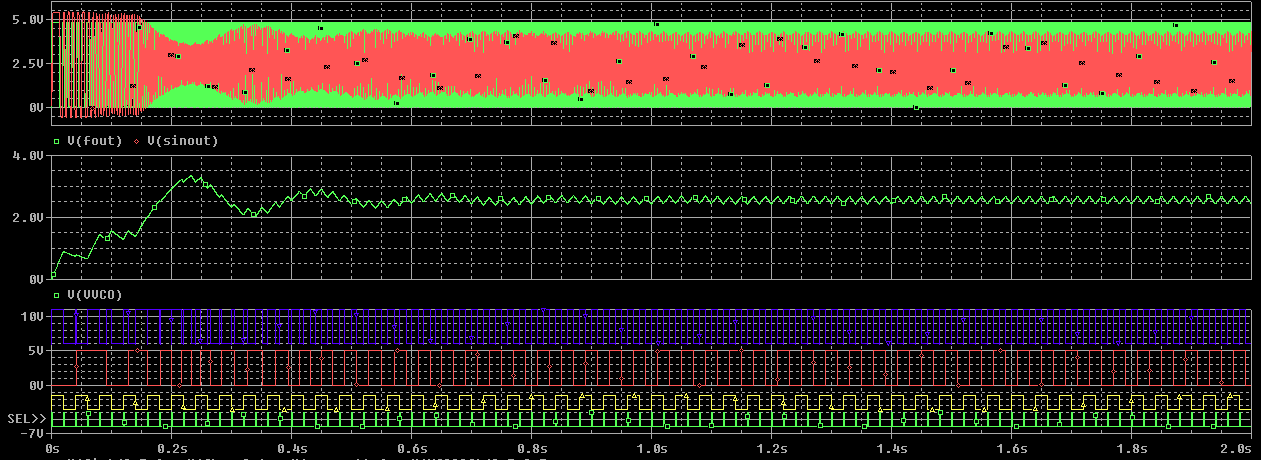
\includegraphics[width=15cm]{pll_2_zoom_full.png}

~

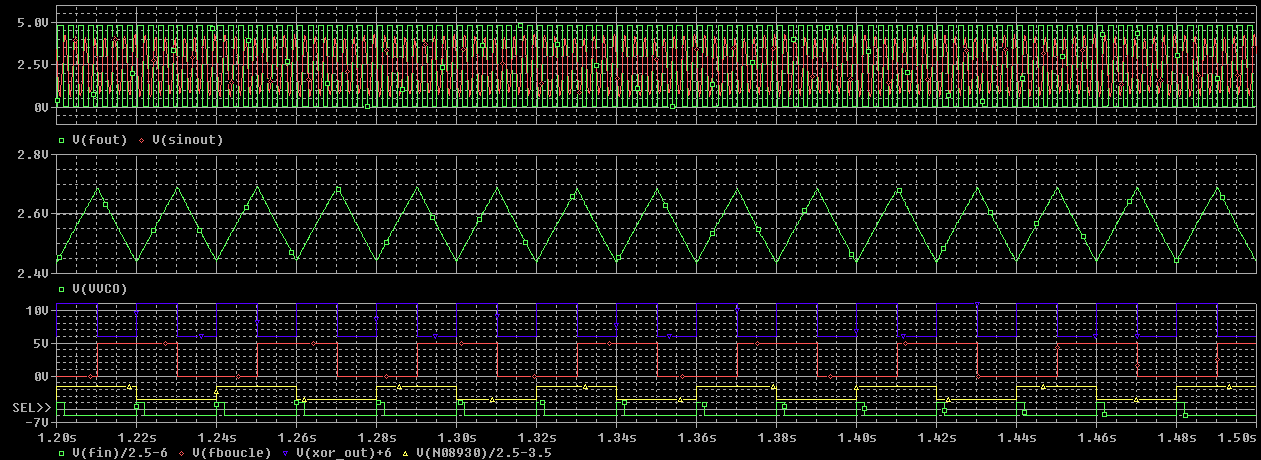
\includegraphics[width=15cm]{pll_2_zoom1.png}

~

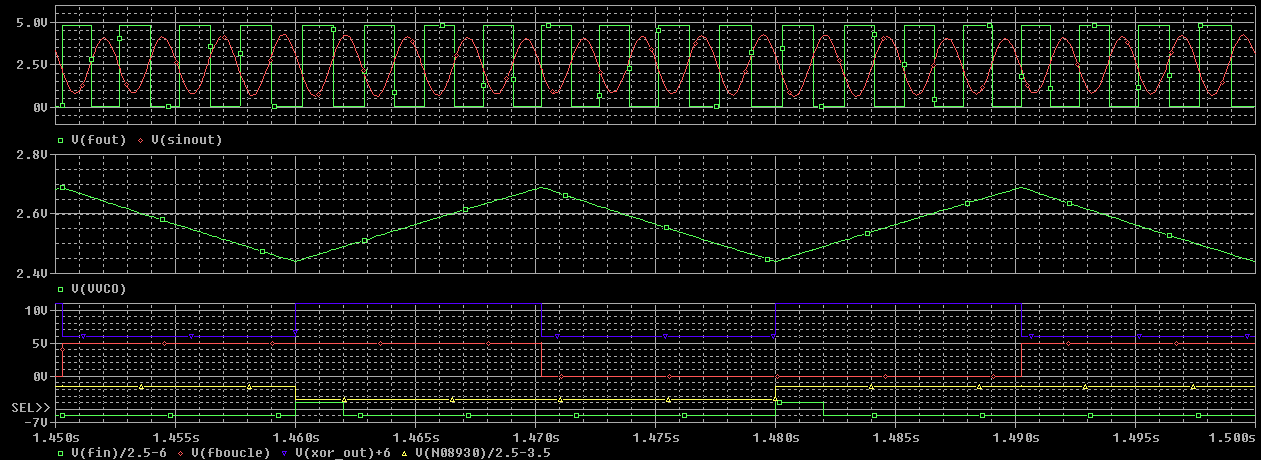
\includegraphics[width=15cm]{pll_2_zoom2.png}

~

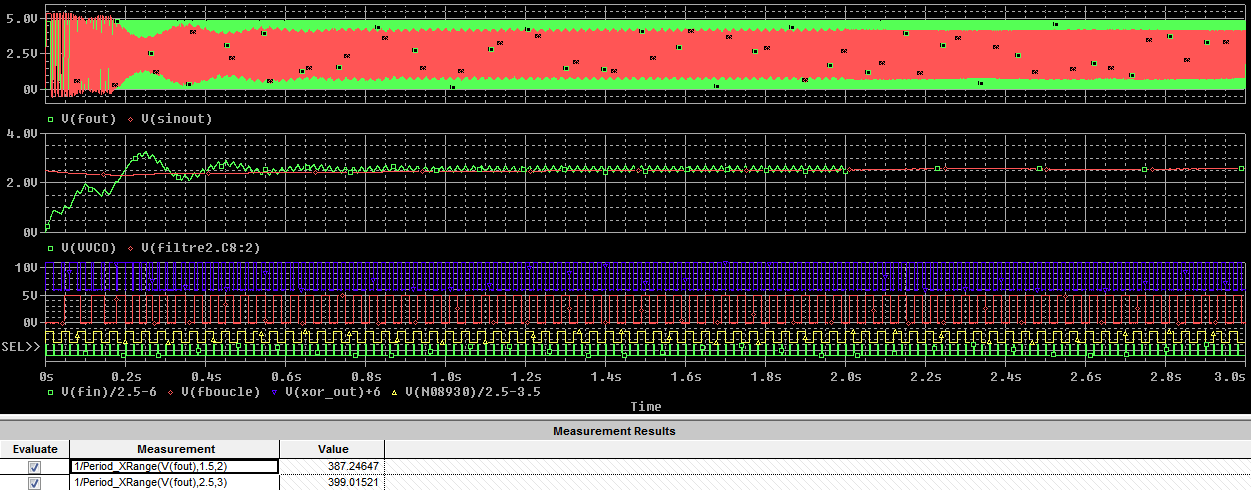
\includegraphics[width=15cm]{pll_3_zoom_full.png}

~

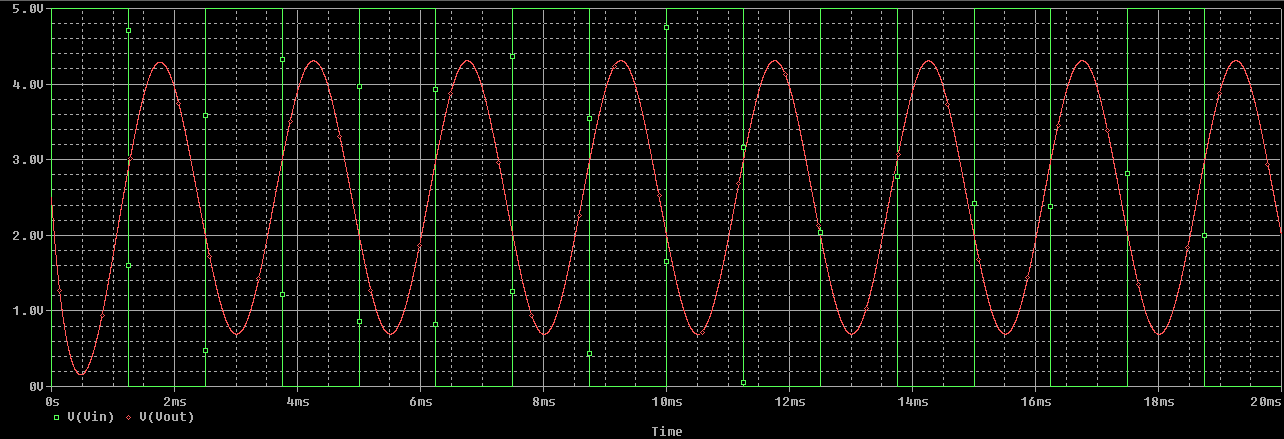
\includegraphics[width=15cm]{trans_filtre_sortie.png}

\section*{Conclusion}

We think we achieved most of what was asked by the client, and maybe a little more with our gates.

~

We also learned a few intersting things, like the difference between an input with a pulse width on 50\% and an input with a random pulse width, or the way to achieve a frequency multiplier.

\end{document}
